%\addcontentsline{toc}{chapter}{Development Process}
\chapter{Final design}
This chapter will give an overview of the final design of the system reached by iteration 10. It will not go into detail for individual parts of the system as these were covered in the iteration chapter but instead will offer a top level perspective of the system.

\section{Overall architecture}
The Laravel framework uses a Model-View-Controller design pattern\cite{mvc} to build applications. It works in the same way as a normal MVC application. Data is stored and manipulated within the models, controllers handle most of the interactions the user has with the system, and the views are the web pages presented to the users. Within Laravel, there is also a front controller, which is used to route incoming HTTP requests to the appropriate views and controllers\cite{Laravel-architechture}.

There are two basic sections of the system, the student end, and the lecturer end. The lecturer end is an admin panel that they can login to, to create and manage their quizzes. The student end consists of the portal for connecting to a session, and the session pages themselves that display the slides and questions for users to answer.

Students only have two bits of functionality available to  them, being able to join a quiz and then being able to answer questions. Lecturers however can do much more on the site. On the admin panel they can create new quizzes, create and add questions to the quizzes and also add slides to the quizzes. They can also change their user details including their session key. The main operation they can perform is that they can run a quiz, this then takes them to the same view as the students, albeit with a small control panel for changing questions or slides, and displaying the results of the quiz. TODO: add final activity diagram, maybe a ui diagram too? See \ref{fig:final-backend-use-case} and \ref{fig:final-frontend-use-case}

\begin{sidewaysfigure}
	\caption{Use case for backend of system}
	\centerline{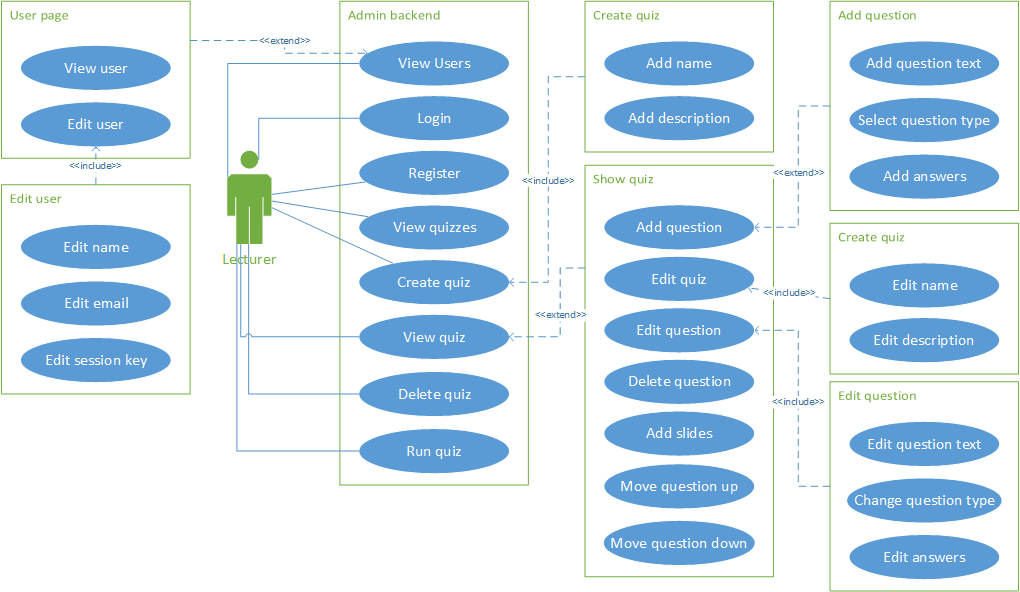
\includegraphics{Chapter3/final-backend-use-case}}
	\label{fig:final-backend-use-case}
\end{sidewaysfigure}

\begin{sidewaysfigure}
	\caption{Use case for frontend of system}
	\centerline{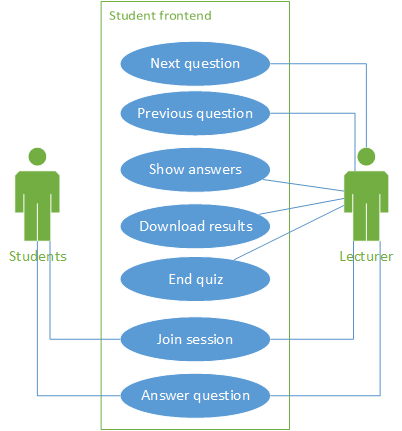
\includegraphics{Chapter3/final-frontend-use-case}}
	\label{fig:final-frontend-use-case}
\end{sidewaysfigure}

\section{Database design}
\begin{figure}
	\caption{Entity relationship digram for final database}
	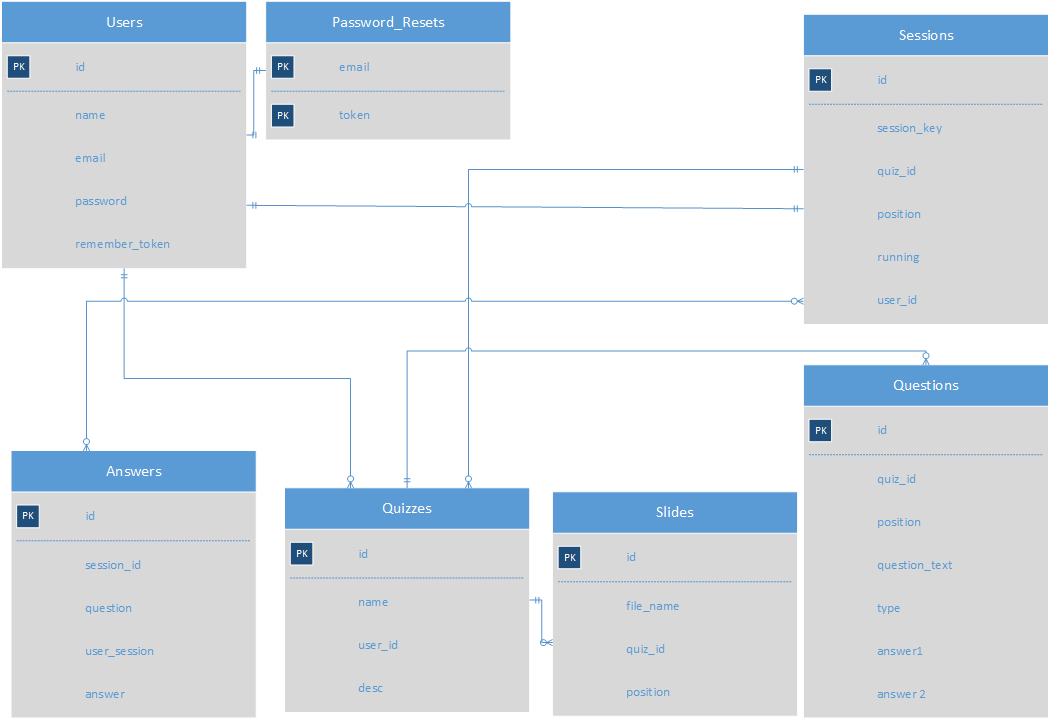
\includegraphics[width=\textwidth]{Chapter3/Final-ER-Image}
	\label{fig:er-diagram}
\end{figure}
\newpage

There are seven tables within the application. Two of these were generated by running a Laravel command to make the authentication part of the site, the users and password\_resets tables. These provide basic user login.

The quizzes table contains information about the quizzes themselves, and are associated with a user. The questions and slides tables both store information about their respective parts of a quiz, with each row within these tables associated with a quiz. Questions store information about the actual question including all the answers, not in the design above are the other eight fields for answers up to answer10. The slides table stores the file name of a slide image that has been converted from a pdf slide. Both of these tables store the positions of their items within a quiz.

The sessions table stores the information about the runnable session, each user has one associated session row. Within this row, the session\_key is stored, which is the key that students would use to connect to a session. Additionally it stores information about the session when its running, specifying if it is running, and what position it is at. This position references the positions specified int he questions and slides tables, though there is no actual foreign key relationship between them. 

The final table, answers, stores all the responses from users to questions. It stores which question, the answer given and the user that submitted the answer. The user\_session is a cookie value rather than a user from the database.
